\documentclass{beamer}

\usetheme{Boadilla}

%\includeonlyframes{current}

\usepackage{bookmark}
\usepackage{times}
\usefonttheme{structurebold}
\usepackage{listings}
\usepackage{ragged2e}

\usepackage{pgf}
\usepackage{tikz}
\usepackage{alltt}
\usepackage[normalem]{ulem}
\usetikzlibrary{arrows}
\usetikzlibrary{automata}
\usetikzlibrary{shapes}
\usepackage{amsmath,amssymb}
\usepackage{rotating}
\usepackage{ulem}
\usepackage{listings}
\usepackage{enumerate}
\usepackage{tikz}
\tikzset{
  every overlay node/.style={
    draw=black,fill=white,rounded corners,anchor=north west,
  },
}
\def\tikzoverlay{%
   \tikz[baseline,overlay]\node[every overlay node]
}%

%\setbeamercovered{dynamic}
\setbeamertemplate{footline}[page number]{}
\setbeamertemplate{navigation symbols}{}
\usefonttheme{structurebold}

\AtBeginSection{\frame{\sectionpage}}

\defbeamertemplate{section page}{mine}[1][]{%
  \begin{centering}
    {\usebeamerfont{section name}\usebeamercolor[fg]{section name}#1}
    \vskip1em\par
    \begin{beamercolorbox}[sep=12pt,center]{part title}
      \usebeamerfont{section title}\insertsection\par
    \end{beamercolorbox}
  \end{centering}
}

\setbeamertemplate{section page}[mine]

\title{Static and Dynamic Analysis of Test Suites}
\author{Patrick Lam}
\date{October 3, 2015}

\colorlet{redshaded}{red!25!bg}
\colorlet{shaded}{black!25!bg}
\colorlet{shadedshaded}{black!10!bg}
\colorlet{blackshaded}{black!40!bg}

\colorlet{darkred}{red!80!black}
\colorlet{darkblue}{blue!80!black}
\colorlet{darkgreen}{green!80!black}

\newcommand{\rot}[1]{\rotatebox{90}{\mbox{#1}}}
\newcommand{\gray}[1]{\mbox{#1}}
\newenvironment{changemargin}[1]{% 
  \begin{list}{}{% 
    \setlength{\topsep}{0pt}% 
    \setlength{\leftmargin}{#1}% 
    \setlength{\rightmargin}{1em}
    \setlength{\listparindent}{\parindent}% 
    \setlength{\itemindent}{\parindent}% 
    \setlength{\parsep}{\parskip}% 
  }% 
  \item[]}{\end{list}}


\lstset{ %
language=C++,
basicstyle=\ttfamily,commentstyle=\scriptsize\itshape,showstringspaces=false,breaklines=true}

\begin{document}

\begin{frame}
  \titlepage
\end{frame}

\begin{frame}
  \frametitle{Goal}
  \Large
  \begin{changemargin}{1cm}
Convince you to analyze programs \emph{and tests} for fun and profit!
  \end{changemargin}
\end{frame}


\begin{frame}
  \centering
  \LARGE
  Why do we analyze programs?
\end{frame}

\begin{frame}
  \frametitle{Why?}
  \Large
  \begin{changemargin}{1cm}
    \begin{itemize}
    \item find bugs;
    \item enable program understanding \& transformation
    \item evaluate software quality
    \end{itemize}
  \end{changemargin}
\end{frame}

% elaborate on these points

\begin{frame}
  \frametitle{Observation}
  \centering
  \LARGE Programs come with gobs of tests.
\end{frame}

\begin{frame}
  \frametitle{Tests and Modern Software}
  Almost-first-class support:\\
  JUnit, etc.

  A form of lightweight specifications.
  \begin{itemize}
  \item executable, provide context
  \item at various granularities (unit, system)
  \end{itemize}
\end{frame}

\begin{frame}
  \frametitle{Pervasiveness of Test Suites}
% add stats
\end{frame}

\begin{frame}
  \frametitle{Opportunity}
  Leverage test suites in program analysis.
\end{frame}

%\begin{frame}
%  \centering \Huge
%  Related Work
%\end{frame}
\section{Related Work}

\begin{frame}
  \frametitle{Static Analysis Limitations}
Soundiness:
\begin{itemize}
\item dynamic class loading
\item eval
\end{itemize}
\end{frame}


\begin{frame}
  \frametitle{Concolic analysis}
\end{frame}

\begin{frame}
  \frametitle{PHP Analysis}

Phantm
\begin{center}

\includegraphics[width=\textwidth]{images/phantm-blue-solid.png}
\end{center}
\begin{itemize}
\item Run the program, observe the configuration loading phase.
\item Use the config to analyze the remainder of the program.
\end{itemize}
\end{frame}

\begin{frame}
  \frametitle{TamiFlex}

\begin{center}

\includegraphics[width=\textwidth]{images/tamiflex.png}
\end{center}
\end{frame}

\begin{frame}
  \frametitle{DSD-Crasher}

\begin{center}
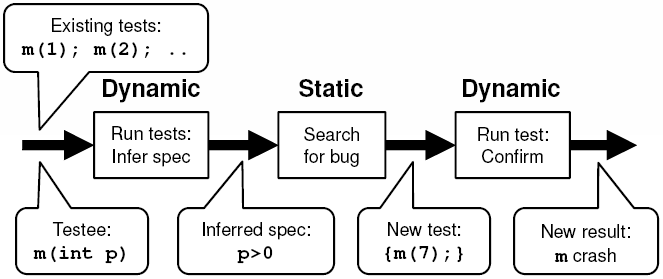
\includegraphics[width=\textwidth]{images/dsd.png}
\end{center}
\end{frame}

\begin{frame}
  \frametitle{Empirical Studies}
\end{frame}

\begin{frame}
  \frametitle{Properties of Test Suites}
  (GTAC 2014)
\end{frame}

\begin{frame}
  \frametitle{Similar Test Methods}
  (PPPJ 2015)
\end{frame}

\section{Future Perspectives}

\begin{frame}
  \frametitle{What Test Suites can Tell Us}
\end{frame}

\begin{frame}
  \frametitle{What We Can Do With Tests?}
\end{frame}

\begin{frame}
  \frametitle{Better Program Understanding via Tests}
\end{frame}

\section{Conclusions}


\end{document}
